\chapter{Specifications}
\label{chapter:specifications}
In this chapter, we describe precisely the IT related specifications (e.g. REST routes, data format, GUI).

%-------------------------------------------------------------------------------
%-------------------------------------------------------------------------------
\section{System architecture}
TODO graphical representation of the system

%-------------------------------------------------------------------------------
%-------------------------------------------------------------------------------
\section{Flow diagram}
The figure~\ref{fig:specs:flowdiagram} defines precisely how the user interacts with the application. It allows to have a clear representation of the system.

\begin{figure}[H]
    \centering
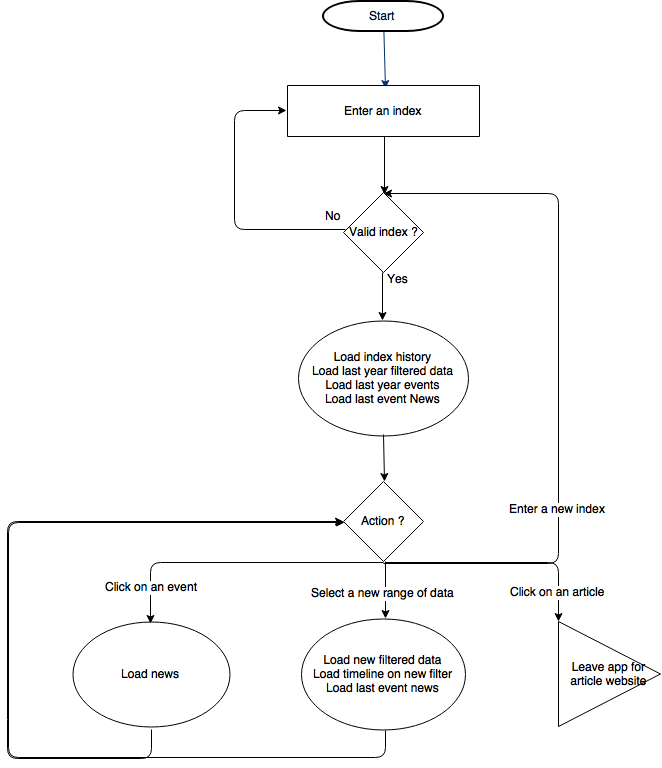
\includegraphics[scale=0.5]{Figures/workflow-stockstrooper.png}
\caption{Flow diagram of the user interaction}
\label{fig:specs:flowdiagram}
\end{figure}

%-------------------------------------------------------------------------------
%-------------------------------------------------------------------------------
\section{REST API}

%-------------------------------------------------------------------------------
\subsection{Routes and format}

\subsubsection*{GET events}
This route sends all events within a period for one index. Default is one year from present. With each event comes its trend. A positive event has a value of \textit{1} and a negative one a value of \textit{-1}.
\begin{verbatim}
/events/:index[/:datestart/:dateend]

[
    {
        "date": "20160502",
        "trends": -1
    },
    {
        "date": "20160716",
        "trends": -1
    },
    {
        "date": "20150123",
        "trends": 1
    }
]
\end{verbatim}

\subsubsection*{GET stocks}
This route sends all the stocks data for one index (market index).
\begin{verbatim}
/stocks/:index

[
      [
            345427200000000000,
            0.426842
      ],
      [
            345686400000000000,
            0.404572
      ],
      [
            345772800000000000,
            0.374879
      ]
]
\end{verbatim}

\subsubsection*{GET news}
This route sends all the news related to one index and one event.
\begin{verbatim}
/news/:index/:dateevent

[
    {
        "url": "http://www.nytimes.com/reuters/2016/01/08/business/
                08reuters-apple-stock-research.html",
        "headline": "Wall St. Bets on Apple Bounceback Despite
                     iPhone Shipment Worries",
        "date": "2016-01-08T09:36:56Z",
        "source": "Reuters"
    }
]
\end{verbatim}

\subsubsection*{GET index valid}
This route sends a boolean variable which indicates if the index is valid or not.
\begin{verbatim}
/index/:index/

{
    "valid": true
}
\end{verbatim}
%-------------------------------------------------------------------------------
\subsection{CORS}

The \textit{CORS} problems were handle with \textit{Flask}.

%-------------------------------------------------------------------------------
\subsection{Detection of events}

The events of a company are detected by searching the biggest changes of share value during a short period of time.

To do this, a threshold is calculated in order to define if the changes of share will be considered as an event.

\begin{lstlisting}[language=python, belowskip=-1.0 \baselineskip]
    threshold = (max(values) - min(values)) * 0.09
\end{lstlisting}

This allows to have a threshold that varies depending on the volatility of the actions. In order to avoid having a threshold to big, the $90\%$ of the calculated value is taken.

Afterwards, we take all the data and process them by samples of a specific size (default value is a size of 10 values). In this current sample, we will calculate the difference between the maximum and the minimal value. If this value exceeds the threshold, this sample will be considered as an event. The sample is composed of multiple dates, the middle date of the sample is chosen to represent the event.

Depending of the stock we are processing, we may have more or less events that we wanted. If we have found more events, we take the highest events and keep them. Events will be sorted by highest difference between max and min value in order to know which ones are the most important. However, if we have less events, the threshold is decrease by $0.05$ and we process all the samples all over again until we have enough events.

This technique is not bulletproof. By processing the values sample by sample, we could miss some events.






